Main entities of the database are:
\begin{itemize}
    \item User;
    \item Event;
    \item Ticket.
\end{itemize}

\subsection{User entity}\label{subsec:user-entity}
User entity, illustrated on a figure~\ref{fig:user_db_1}, represents user in the database and have several fields:

\begin{center}
    \begin{tabular}{ | c | c | c | c | }
        \hline
        \textbf{Name}          & \textbf{Type}    & \textbf{Description}                 & \textbf{Constraints}                         \\ \hline
        \texttt{id}            & \textit{integer} & unique identifier of the user        & \textbf{\color{red}Primary Key}              \\ \hline
        \texttt{name}          & \textit{text}    & name of the user                     & \textbf{\color{blue}Unique}                  \\ \hline
        \texttt{email}         & \textit{text}    & email of the user                    & \textbf{\color{blue}Unique}                  \\ \hline
        \texttt{created\_date} & \textit{text}    & date of instance creation in the UTC & \multirow{2}{*}{\textbf{N\textbackslash{A}}} \\ \cline{0-2}
        \texttt{updated\_date} & \textit{text}    & date of the last update in the UTC   &                                              \\ \hline
    \end{tabular}
\end{center}

Indexes for user entity:

\begin{center}
    \begin{tabular}{ | c | c | }
        \hline
        \textbf{Name}  & \textbf{Type}   \\ \hline
        \texttt{name}  & \textit{B-tree} \\ \hline
        \texttt{email} & \textit{B-tree} \\ \hline
    \end{tabular}
\end{center}

\begin{figure}[h]
    \label{fig:user_db_1}
    \centering
    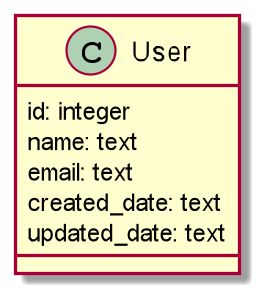
\includegraphics[width=0.35\textwidth]{images/user}
    \caption{User representation in the database}
\end{figure}

\subsection{Event entity}\label{subsec:event-entity}

Event entity, illustrated on a figure~\ref{fig:event_db_1} , represents event in the database and have several fields:

\begin{center}
    \begin{tabular}{ | c | c | c | c |}
        \hline
        \textbf{Name}          & \textbf{Type}    & \textbf{Description}                 & \textbf{Constraints}                         \\ \hline
        \texttt{id}            & \textit{integer} & unique identifier of the event       & \textbf{\color{red}Primary Key}              \\ \hline
        \texttt{title}         & \textit{text}    & title of the event                   & \multirow{2}{*}{\textbf{\color{blue}Unique}} \\ \cline{0-2}
        \texttt{date}          & \textit{text}    & start date of the event in the UTC   &                                              \\ \hline
        \texttt{created\_date} & \textit{text}    & date of instance creation in the UTC & \multirow{2}{*}{\textbf{N\textbackslash{A}}} \\ \cline{0-2}
        \texttt{updated\_date} & \textit{text}    & date of the last update in the UTC   &                                              \\ \hline
    \end{tabular}
\end{center}

Indexes for event entity:

\begin{center}
    \begin{tabular}{ | c | c | }
        \hline
        \textbf{Name}  & \textbf{Type}   \\ \hline
        \texttt{title}  & \textit{B-tree} \\ \hline
        \texttt{date} & \textit{B-tree} \\ \hline
    \end{tabular}
\end{center}

\begin{figure}[h]
    \centering
    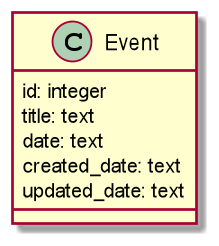
\includegraphics[width=0.35\textwidth]{images/event}
    \caption{Event representation in the database}
    \label{fig:event_db_1}
\end{figure}

\subsection{Ticket entity}\label{subsec:ticket-entity}

Ticket entity, illustrated on a figure~\ref{fig:ticket_db_1} , represents ticket in the database and have several fields:

\begin{center}
    \begin{tabular}{ | c | c | c | c | c |}
        \hline
        \textbf{Name} & \textbf{Type} & \textbf{Description} & \multicolumn{2}{c|}{\textbf{Constraints}} \\ \hline
        \texttt{id} & \textit{integer} & unique identifier of the ticket & \multicolumn{2}{c|}{\textbf{\color{red}Primary Key}} \\ \hline
        \texttt{user\_id} & \textit{integer} & id of the user which has ordered this ticket & \multicolumn{2}{c|}{\textbf{\color{SecondaryKeyColor}Secondary Key}} \\ \hline
        \texttt{event\_id} & \textit{integer} & id of the event on which ticket is booked & \textbf{\color{SecondaryKeyColor}Secondary Key}  & \multirow{2}{*}{\textbf{\color{blue}Unique}} \\ \cline{0-3}
        \texttt{place}     & \textit{integer} & number of place of the ticket             & \textbf{N\textbackslash{A}}                                     &                                              \\ \hline
        \texttt{category} & \textit{string} & category of the ticket & \multicolumn{2}{c|}{\multirow{3}{*}{\textbf{N\textbackslash{A}}}} \\ \cline{0-2}
        \texttt{created\_date} & \textit{string} & date of instance creation in the UTC & \multicolumn{2}{c|}{} \\ \cline{0-2}
        \texttt{updated\_date} & \textit{string} & date of the last update in the UTC & \multicolumn{2}{c|}{} \\ \hline
    \end{tabular}
\end{center}

Indexes for ticket entity:

\begin{center}
    \begin{tabular}{ | c | c | }
        \hline
        \textbf{Name}  & \textbf{Type}   \\ \hline
        \texttt{event\_id}  & \textit{B-tree} \\ \hline
        \texttt{user\_id}  & \textit{B-tree} \\ \hline
        \texttt{category} & \textit{B-tree} \\ \hline
    \end{tabular}
\end{center}

\begin{figure}[h]
    \centering
    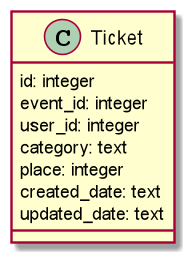
\includegraphics[width=0.35\textwidth]{images/ticket}
    \caption{Ticket representation in the database}
    \label{fig:ticket_db_1}
\end{figure}